%%% Intro.tex --- 
%% 
%% Filename: Intro.tex
%% Description: 
%% Author: Ola Leifler
%% Maintainer: 
%% Created: Thu Oct 14 12:54:47 2010 (CEST)
%% Version: $Id$
%% Version: 
%% Last-Updated: Thu May 19 14:12:31 2016 (+0200)
%%           By: Ola Leifler
%%     Update #: 5
%% URL: 
%% Keywords: 
%% Compatibility: 
%% 
%%%%%%%%%%%%%%%%%%%%%%%%%%%%%%%%%%%%%%%%%%%%%%%%%%%%%%%%%%%%%%%%%%%%%%
%% 
%%% Commentary: 
%% 
%% 
%% 
%%%%%%%%%%%%%%%%%%%%%%%%%%%%%%%%%%%%%%%%%%%%%%%%%%%%%%%%%%%%%%%%%%%%%%
%% 
%%% Change log:
%% Completed Language Reading MBS
%% 
%% RCS $Log$
%%%%%%%%%%%%%%%%%%%%%%%%%%%%%%%%%%%%%%%%%%%%%%%%%%%%%%%%%%%%%%%%%%%%%%
%% 
%%% Code:


\chapter{Advanced Modeling Simulation Analysis}
\label{cha:python}


This chapter is based on the following papers:

\begin{itemize}
		
	\item Bernt Lie, Sudeep Bajracharya, \textbf{Alachew Mengist}, Lena Buffoni, Arun Kumar, Martin Sj\"{o}lund, Adeel Asghar, Adrian Pop, Peter Fritzson.\textbf{ API for Accessing OpenModelica Models From Python.} In Proceedings of 9th EUROSIM Congress on Modeling and Simulation, September 12-16, 2016, Oulu, Finland. 
	
	\item Adeel Asghar, Andreas Pfeiffer, Arunkumar Palanisamy, \textbf{Alachew Mengist}, Martin Sj\"{o}lund, Adrian Pop and Peter Fritzson.\textbf{ Automatic Regression Testing of Simulation Models and Concept for Simulation of Connected FMUs in PySimulator.} In Proceedings of the 11th International Modelica Conference, Versailles, France, September 21-23, 2015. 
		
\end{itemize}

\section{Introduction}
\label{sec:pythonintroduction}

EOO languages such as Modelica have relatively little support for the advanced model analysis and synthesis needed for control systems design, particularly for optimal control problems (OCPs). Examples of such desirable analysis capabilities include (i) study of model sensitivity, (ii) random number generation and statistical analysis, (iii) Monte Carlo simulation, (iv) advanced plotting capabilities, (v) general optimization capabilities, (vi) linear analysis and control synthesis, etc. Scripting languages such as MATLAB and Python include most of these desirable analytical capabilities, and it is of interest to integrate Modelica models with such scripting languages. For the purposes of this work, we have chosen to use Python and OpenModelica due to their open-source availability.

A Python API for controlling Modelica simulation and analysis from Python was proposed in February 2015\footnote{Python API for Accessing OpenModelica Models, by B. Lie, February 20, 2015.}. Based on this proposal, we have developed an initial version of a Python API for operating on Modelica models in Python. In this chapter, we present how to generate a Python object from an EOO Modelica model, how to set operating conditions, and how to run the simulation to produce a result object. Furthermore, we describe how to carry out linearization of a model object, the possibility of carrying out parameter sensitivity studies, and how to extract results from the result object to Python. The proposed solution has been tested on several industrially-relevant models, and its use for automatic analysis of Modelica models from Python is illustrated using a simple water tank model.

\section{Description of the API}
\label{sec:pythonapi}

The API is described in the subsections below.

\subsection{Python Class and Constructor}
\label{subsec:pythonclass}

The name of the Python class that is used for operation on Modelica models is \textit{ModelicaSystem}.
This \textit{class} is equipped with an object constructor with the same name as the class. In addition, the class is equipped
with a number of methods for manipulating the instantiated objects. In this subsection, we discuss how to import the class, and
how to use the constructor to instantiate an object. The object is imported from package OMPython, i.e., with
Python commands.

\begin{lstlisting}
  >>>from OMPython import ModelicaSystem
\end{lstlisting}

Other Python packages to be used, such as \textit{numpy},\textit{matplotlib}, \textit{pandas}, etc. must be imported in a similar
manner. The object constructor requires a minimum of 2 input arguments which are strings, and may need a third string input
argument.

\begin{itemize}
	\item The \textit{first input argument} must be a string with the file name of the Modelica code, with Modelica file extension\textit{.mo}. If the 	 
	       Modelica file is not in the current directory of Python, then the file path must also be included.
	\item The \textit{second input argument} must be a string with the name of the Modelica model, including the namespace if the model is wrapped 
		  within a Modelica package.
	\item A \textit{third input argument} is used if the Modelica model builds on other Modelica code, e.g., the Modelica Standard Library.
\end{itemize}

Example 1: Use of constructor. Suppose we have a Modelica model with name CSTR wrapped in a Modelica package \textit{Reactors} — stored in file
\textit{Reactor.mo}:

\begin{lstlisting}
package Reactors
	// ...
	model CSTR
		/// ...
	end CSTR;
	//
end Reactors;
\end{lstlisting}

If this model does not use any external Modelica code and the file is located in the current Python directory, the following
Python code instantiates a Python object \textit{mod}:

\begin{lstlisting}
>>> mod = ModelicaSystem('Reactors.mo','Reactors.CSTR')
\end{lstlisting}

The user is free to choose any valid Python label name for the Python object. All methods of class \textit{ModelicaSystem} refers to the instantiated object, in standard Python fashion. Thus, method \textit{simulate()} is invoked with the Python command:

\begin{lstlisting}
>>>mod.simulate()
\end{lstlisting}

In the subsequent overview of methods, the object name is not included. In practice, of course, it must be included in order
to operate on the object in question. Methods may have no input arguments, one, or several input arguments. Methods may or may not return results — if the methods do not return results, the results are stored within the object.

\subsection{Utility routines, converting Modelica $\leftrightarrow$ FMU:}
\label{subsec:pythonmodelicafmu}
Two utility methods convert files between Modelica files with file extension \textit{.mo} and Functional Mock-up Unit (FMU) files with
file extension \textit{.fmu}.

\begin{enumerate}
	\item \textit{convertMo2Fmu()} — method for converting the Modelica model of the object, say ModelName, into FMU file.
	\begin{itemize}
		\item Required input arguments: none, operates on the Modelica file associated with the object.
		\item Optional input arguments:
		\begin{itemize}
			\item \textit{className}: string with the class name that should be translated,
			\item \textit{version}: string with FMU version, "1.0" or "2.0"; the default is "1.0".
			\item \textit{fmuType}: fmuType: string with FMU type, "me" (model exchange) or "cs" (co-simulation); the default is "me".
			\item \textit{fileNamePrefix}: string; the default is \'className\'.
			\item \textit{generatedFileName}: string, returns the full path of the generated FMU.
		\end{itemize}
		\item Result: file \textit{ModelName.fmu} in the current directory
	\end{itemize}
	\item \textit{convertFmu2Mo(s)} — method for converting an FMU file into a Modelica file.
	\begin{itemize}
		\item Required input arguments: string s, where s is the name of an FMU file, including extension \textit{.fmu}.
        \item Optional input arguments: a number of optional input arguments, e.g., the possibility to change working directory for the imported FMU files.
        \item Result: Assume the name of the file is \textit{fmuName.fmu}. Then file \textit{fmuName\_me\_FMU.mo} is generated in the current Python  
        	  directory.
	\end{itemize}
	\item \textit{Getting and setting information:} Quite a few methods are dedicated to getting and setting information about
	objects. With two exceptions — \textit{getQuantities()} and \textit{getSolutions()} — the use of input arguments and results is identical for all get methods, while input arguments are used identically for all of the set methods, with results	stored in the object.
	
	The Method \textit{getQuantities()} does not accept input arguments, and returns a list of dictionaries, one dictionary for each
	quantity. Each dictionary has the following keys — with values being strings, too.
	\begin{itemize}
		\item \textit{Changeable} — value \textit{'true'} or \textit{'false'},
		\item \textit{Description} — the string used in Modelica to describe the quantity, e.g., \textit{'Mass in tank, kg'},
		\item \textit{Name} — the name of the quantity, e.g., \textit{'T', 'der(T)', 'n[1]', 'mod1.T'}, etc.,
		\item \textit{Value} — the value of the quantity, e.g., \textit{'None', '5.0'}, etc.,
		\item \textit{Variability} — \textit{'continuous','parameter'}.
    \end{itemize}
	When applying the \textit{Pandas method DataFrame} to the returned list of dictionaries, the result is a conveniently
	typeset table in Jupyter notebooks. Modelica \textit{constants} are not included in the returned quantities. Standard get 
	methods \textit{getXXXs()}, where \textit{XXXs} is in	\textit{{Continuous, Parameters, Inputs, Outputs,SimulationOptions, OptimizationOptions,LinearizationOptions}} are considered. Thus, methods \textit{getContinuous(), getParameters()}, etc.
	Two Standard get methods are accepted.
	\begin{itemize}
		\item \textit{getXXXs()}, i.e., without input argument, returns a dictionary with names as keys and values as ... values.
		\item \textit{getXXXs(S)}, where S is a sequence of strings of names, returns a tuple of values for the specified names.
    \end{itemize}
	Getting solutions: We consider method getSolutions(). Two calling possibilities are accepted.
	\begin{itemize}
		\item \textit{getSolutions()}, i.e., without input arguments, returns a list of strings of names of quantities for
			          which there is a solution = time series.
		\item \textit{getSolutions(S)}, where S is a sequence of strings of names, returns a tuple of values = 1D
					numpy arrays = time series for the specified names.
	\end{itemize}
	Setting methods: We consider the method \textit{setXXXs()} to set the information, where \textit{XXXs} is in \textit{(Parameters, Inputs, SimulationOptions, OptimizationOptions,
	LinearizationOptions=, thus methods setParameters(), setInputs()}, etc. Two calling possibilities are accepted.
	\begin{itemize}
		\item \textit{setXXXs(K)}, with K being a sequence of keyword assignments of type \textit{quantity name = value}. Here, the quantity name could  
		         be a parameter name (i.e., not a string), an input name, etc.
       \begin{itemize}
         	\item For parameters and simulation/optimization/linearization options, the value should be a numerical value or a string
         		(e.g., a string of ODE solver name such as \textit{'dassl'}, etc.).
         	\item For inputs, the value could be a numerical value if the input is constant in the time range of the simulation,
         	\item For inputs, the value could alternatively be a list of tuples $(t_j, u_j)$, i.e., $[(t_1, u_1) , (t_2, u_2) ,...., (t_N, u_N)]$ where the input varies linearly between $(t_j ; u_j)$ and $(t_{j+1}, u_{j+1})$, where $t_j \leq t_{j+1}$, and where
         	at most two subsequent time indices $t_j, t_{j+1}$ can have the same value. As an example, $[..., (1,10), (1,20), ...] $ describes a perfect jump in input value from value 10 to value 20 at time instance 1.
         	\item This type of sequence of input arguments does not work for certain quantity names, e.g.,\textit{'der(T)', 'n[1]', 'mod1.T'}, because
         		Python does not allow for label names \textit{der(T), n[1], mod1.T}, etc.
       \end{itemize}
		         
		\item \textit{setXXXs(**D)}, with \textit{D } being a \textit{dictionary} with quantity names as keywords and values as described
			with the alternative input argument \textit{K}.
	\end{itemize}
	
	\item \textit{Operating on Python object: simulation, optimization:} The following methods operate on the object, and
	have no input arguments. The methods have no return values, instead the results are stored within the object. To retrieve the results, method 	\textit{getSolutions()} is used, as described previously.
	\begin{itemize}
		\item \textit{simulate()} — simulates the system with the given simulation options.
		\item \textit{optimize()} — optimizes the Optimica problem with the given optimization options.
	\end{itemize}

	\item \textit{Operating on Python object: linearization:} The following methods are proposed for linearization:
	\begin{itemize}
		\item \textit{linearize()} — with no input argument, returns a tuple of 2D numpy arrays (matrices) A, B, C and D.
		\item \textit{getLinearInputs()} — with no input argument, returns a list of strings of names of inputs used when forming matrices B and D.
		\item \textit{getLinearOutputs()} — with no input argument, returns a list of strings of names of outputs used when forming matrices C and D.
		\item \textit{getLinearStates()} — with no input argument, returns a list of strings of names of states used when forming matrices A, B, C and
	\end{itemize}
\end{enumerate}

\section{Case Study: Python API usage for Model Analysis}
\label{subsec:pythoncasestudy}

We consider the simple tank in Figure \ref{fig:pythonwatertankmodel} filled with water. Water with initial mass $m(0)$ is emptied by gravity
through a hole in the bottom at effluent mass flow rate $\dot{m}_e$, while at the same time water is filled into the tank at influent mass flow rate $\dot{m}_i$.

\begin{figure}
	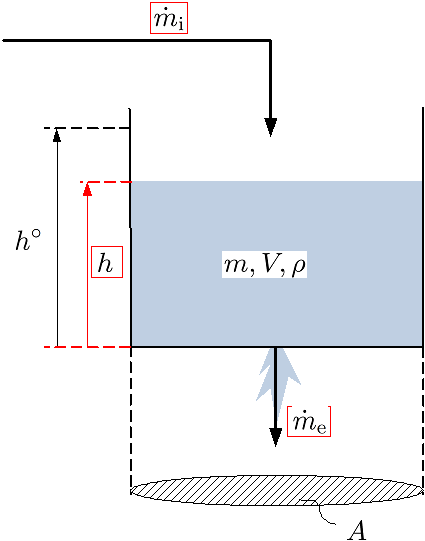
\includegraphics[width=\linewidth]{python_water_tank_model.png}
	\caption{Driven water tank, with externally available quantities framed	in red: initial mass is emptied through bottom at rate $\dot{m}_e $, while at the same time water enters the tank at rate $\dot{m}_i$ }
	\label{fig:pythonwatertankmodel}
\end{figure}

Our modeling objective is to find the liquid level h. This objective is illustrated by the functional diagram in
Figure \ref{fig:pythonwatertankfunctional}. The functional diagram depicts the causality of the system (“Tank with influent and effluent mass flow”), where inputs (green arrow) cause a change in the system and its output (orange arrow)\footnote{Although Modelica is an acausal modeling language, it is useful to think in terms of causality during model development.}. Here, the input variable is the influent mass flow rate $\dot{m}_i$, while the output variable is the quantity we are interested in, $h$.

\begin{figure}
	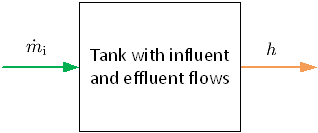
\includegraphics[width=\linewidth]{python_water_tank_functional.png}
	\caption{Functional diagram of tank with influent and effluent flow.}
	\label{fig:pythonwatertankfunctional}
\end{figure}

\subsection{Model Summary}
\label{subsec:pythonmodelsummary}

The model can be summarized in a form suitable for implementation in Modelica as:

\begin{equation*}
	\begin{aligned}
	    \frac{d_m}{d_t} = \dot{m}_i - \dot{m}_e \\
	     m = pV \\
	     V = Ah \\
	     \dot{m}_e = K\sqrt{\frac{h}{h^{\nabla^.}}} 
	\end{aligned}
\end{equation*}

To complete the model description, we need to specify model parameters and operating conditions. Model parameters
(constants) are given in Table \ref{tab:tablemodelparameters}, and the operating conditions are given in Table \ref{tab:tablemodeloperatingconditions}.

\begin{table}
	\begin{center}
		\caption{Parameters for driven tank with constant cross sectional area.} 
		\label{tab:tablemodelparameters} 
		\begin{tabular}{ cccc } 
			\hline
			\bfseries Parameter & \bfseries Value  & \bfseries Unit  & \bfseries Comment \\ 
			$p$ & $1$ & $kg/L $ & Density of liquid \\ 
			$A$ & $5$ & $dm^2$ & Constant cross sectional area \\ 
			$K$ & $5$ & $kg/s$ & Valve constant \\
			$h^{\nabla}$ & $3$ & $dm$ & Level scaling \\  
			\hline
		\end{tabular}
	\end{center}
\end{table}

\begin{table}
	\begin{center}
		\caption{Operating condition for driven tank with constant cross sectional area.} 
		\label{tab:tablemodeloperatingconditions} 
		\begin{tabular}{ cccc } 
			\hline
			\bfseries Quantity & \bfseries Value  & \bfseries Unit  & \bfseries Comment \\ 
			$h(0)$ & $1.5$ & $dm $ & Initial level \\ 
			$m(0)$ & $ph (0) A $ & $kg$ & Initial mass \\ 
			$\dot{m}_i (t)$ & $2$ & $kg/s$ & Nominal influent mass flow rate; may be varied \\
			\hline
		\end{tabular}
	\end{center}
\end{table}

\subsection{Water Tank Model expressed in Modelica}
\label{subsec:pythonmodleicamodel}

The Modelica code describes the core model of the tank, \textit{ModWaterTank}, and consists of a first section where
constants and variables are specified, and a second section where the model equations are specified.

\begin{lstlisting}
	model ModWaterTank 
		// Main driven water tank model 
		// author: Bernt Lie 
		// University College of 
		// Southeast Norway 
		// April 18, 2016 
		//
		// Parameters
		constant Real rho = 1 "Density";
		parameter Real A = 5 "Tank area";
		parameter Real K = 5 "Valve const";
		parameter Real h\_max = 3 "Scaling";
		// Initial state parameters
		parameter Real h\_0 = 1.5 "Init.level";
		parameter Real m\_0 = rho*h\_0*A "Init.mass";
		// Declaring variables
		// -- states
		Real m(start = m\_0, fixed = true) "Mass in tank, kg";
		// -- auxiliary variables
		Real V "Tank liquid volume, L";
		Real md\_e "Effluent mass flow";
		// -- input variables
		input Real md\_i "Influent mass flow";
		// -- output variables 
		output Real h "Tank liquid level,dm";
		// Equations constituting the model 
		equation 
		// Differential equation 
		der(m) = md\_i - md\_e; 
		// Algebraic equations 
		m = rho*V; 
		V = A*h;
		md\_e = K*sqrt(h/h\_max);
	end ModWaterTank;
\end{lstlisting}

As seen from the first section of model \textit{ModWaterTank}, the model has 4 essential parameters
$(rho-h_max)$, one of which is a Modelica constant $(rho)$ while the other 3 are design parameters (compare this
to Table I). Furthermore, the model contains 2 "initial state" parameters, where 1 of them can be chosen at
liberty, $h_0$, while the other one, $m_0$, is computed automatically from $h_0$, see Table II. The purpose of
the "free parameter" $h_0$ is that it is easier for the user to specify level than mass. Also, free "initial state"
parameters make it possible for the user to change the initial states from outside of model ModWaterTank, e.g., from Python.

Next, one variable is given with an initial value — the state $m$ — which is initialized with the "initial state" parameter
$m_0$. Then, 2 variables are defined as auxiliary variables (algebraic variables), $V$ and $md_e$\footnote{$md$ is notation for $m$ with a dot, $\dot{m}$ , i.e., a mass flow rate.}

One input variable is defined — $md_i$ — which is the influent mass flow rate $\dot{m}_i$, see Table \ref{tab:tablemodeloperatingconditions}. Inputs have the characteristic that their values are not specified in the core model — here\textit{ModWaterTank}. Instead,
their values must be given in an external model/code — we will specify this input in Python. Finally, 1 output is
given — $h$.

In the second section of model \textit{ModWaterTank}, the model equations exactly map the mathematical model
given in Section \ref{subsec:pythonmodelsummary}. For purposes of illustration, the core model \textit{ModWaterTank} is wrapped within a package named
\textit{WaterTank} and stored in file \textit{WaterTank.mo},


\begin{lstlisting}
	package WaterTank
		// Package for simulating
		// driven water tank
		// author: Bernt Lie
		// University College of
		// Southeast Norway
		// April 18, 2016
		//
		model ModWaterTank
		// Main driven water tank model
		// ....
		....
		end ModWaterTank;
		// End package
	end WaterTank;
\end{lstlisting}

\subsection{Use of Python API}
\label{subsec:pythonuseapi}

First, for example on Jupyter notebook, the following Python statements are executed:

\begin{lstlisting}
	from OMPython import ModelicaSystem
	import numpy as np
	import numpy.random as nr
	%matplotlib inline
	import matplotlib.pyplot as plt
	import pandas as pd
	LW = 2
\end{lstlisting}

Here, we use \textit{NumPy} to handle simulation results, etc. The random number package will be used in
a sensitivity/Monte Carlo study. The \textit{magic} function \textit{\%matplotlib inline} is used to embed Matplotlib
plots within the Jupyter notebook; to save these plots into files, simply right-click the plots. However, more options
for saving files are available if the magic function is \textit{excluded}, and the \textit{plt.show()} command is instead added
after the plot commands have been completed. The pandas library is used to illustrate presenting data in tables in a Jupyter
notebook. Finally, label \textit{LW} is used to give a conform line width in plots.

\subsection{Basic Simulation of Model}
\label{subsec:pythonsimulatemodel}

We instantiate object \textit{tank} by running the \acrshort{omc} Server with the following command:

\begin{lstlisting}
	tank = ModelicaSystem('WaterTank.mo','WaterTank.ModWaterTank')
\end{lstlisting}

Next, we are interested in which \textit{quantities} are available in the model. Python prompt \textit{>>>} is used when Jupyter
notebook actually uses \textit{In[*]} — where \textit{*} is some number, while the response in Jupyter notebook is prepended
with \textit{Out[*]}.

\begin{lstlisting}
	>>> q = tank.getQuantities()
	>>> type(q)
	list
	>>> len(q)
	11
	>>> q[0]
	{'Changeable': 'true', 
	'Description': 'Mass in tank, kg',
	'Name': 'm',
	'Value': None,
	'Variability': 'continuous'}
	>>> pd.DataFrame(q)
\end{lstlisting}

The last command leads Jupyter notebook to typeset a tabular presentation of the quantities, Figure \ref{fig:pythontypesetting}. The results
in Figure \ref{fig:pythontypesetting} should be compared to the Modelica model in \ref{subsec:pythonmodleicamodel}. Observe that Modelica \textit{constants} are not included in the quantity list.

\begin{figure}
	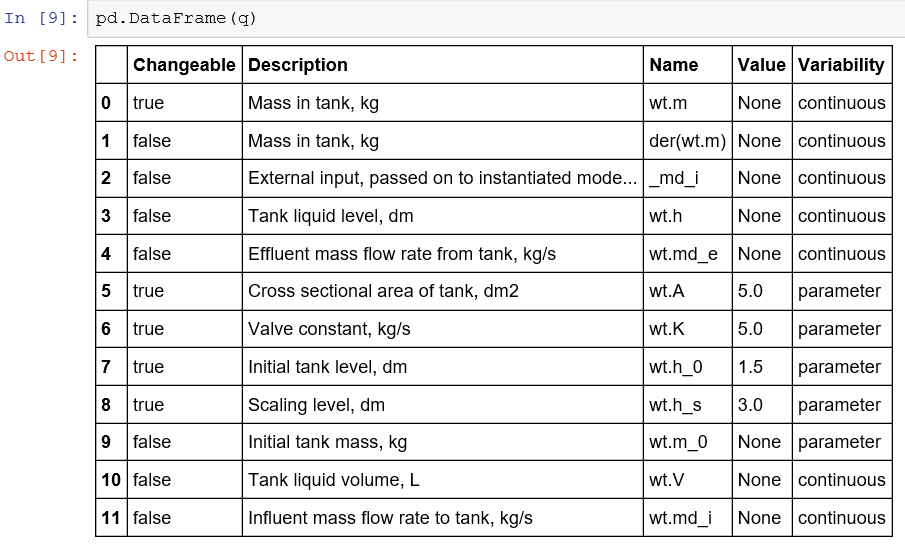
\includegraphics[width=\linewidth]{python_typesetting.png}
	\caption{Typesetting of Data Frame of quantity list in Jupyter notebook.}
	\label{fig:pythontypesetting}
\end{figure}

Next, we check the simulation options:

\begin{lstlisting}
	>>> tank.getSimulationOptions()
	{'solver': 'dassl',
	'startTime': 0.0,
	'stepSize': 0.002,
	'stopTime': 1.0,
	'tolerance': 1e-06}
\end{lstlisting}

It should be observed that the \textit{stepSize} is the frequency at which solutions are stored, and is not the step
size of the solver. The number of data points \textit{stored} is thus \textit{(stopTime-startTime)/stepSize} with appropriate
rounding. This means that if we increase the \textit{stopTime} to a large number, we should also increase the \textit{stepSize} to
avoid storing a large volume of information.


To this end, we want to simulate the system for a long time, until the level reaches a steady state. Possible inputs are:

\begin{lstlisting}
	>>> tank.getInputs(){'md_i': None}
\end{lstlisting}

where value None implies that the available input, $md_i$, has not yet been set. We could use \textit{None} as input, which will be interpreted as zero. 
But let us instead set $\dot{m}_i = 3$, simulate for a long time, and change the "initial state"
parameter $h (0)$ to the steady state value of $h$:

\begin{lstlisting}
	>>> tank.setInputs(md_i=3)
	>>> tank.setSimulationOptions\
	(stopTime=1e4, stepSize=10)
	>>> tank.simulate()
	>>> h = tank.getSolutions('h')
	>>> tank.setParameters(h_0 = h[-1])
\end{lstlisting}

Next, we set back the stop time to 10, and specify an input sequence with a couple of jumps:

\begin{lstlisting}
	>>> tank.setSimulationOptions\(stopTime=10, stepSize=0.02)
	>>> tank.setInputs(md_i = [(0,3),(2,3),(2,4),(6,4),(6,2),(10,2)])
\end{lstlisting}

Finally, we simulate the model with the time varying input, and plot the result:

\begin{lstlisting}
	>>> tank.simulate()
	>>> tm, h = tank.getSolutions('time','h')
	>>> plt.plot(tm,h,linewidth=LW,color='blue', label=r'$h$')
	>>> plt.title('Water tank level')
	>>> plt.xlabel(r'time $t$ [s]')
	>>> plt.ylabel(r'$h$ [dm]')
\end{lstlisting}

The result is displayed in Figure \ref{fig:pythonwatertanklevelplot}.

\begin{figure}
	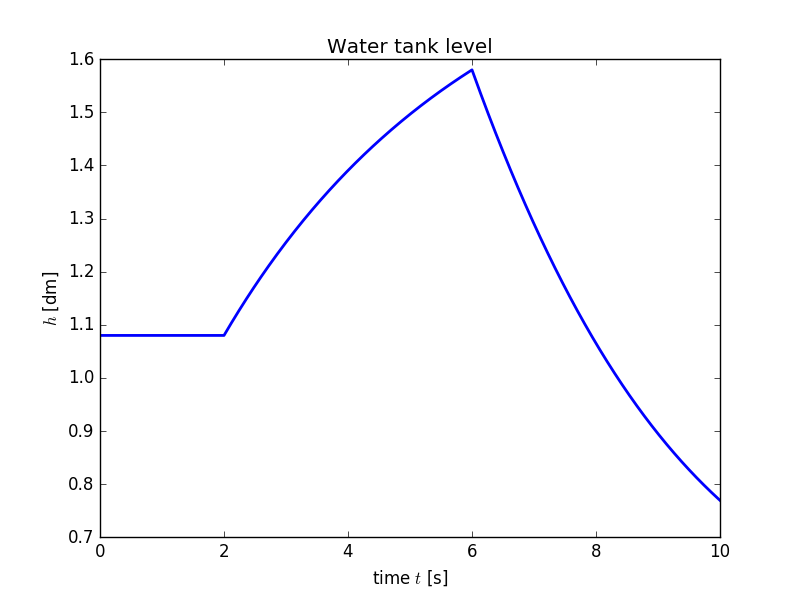
\includegraphics[width=\linewidth]{python_water_tank_level_plot.png}
	\caption{Tank level when starting from steady state, and $\dot{m}_i(t)$ varies in a straight line between the points $(tj,\dot{m}_i(t_j ))$
		given by the list $[(0; 3); (2; 3); (2; 4); (6; 4); (6; 2); (10; 2)]$.}
	\label{fig:pythonwatertanklevelplot}
	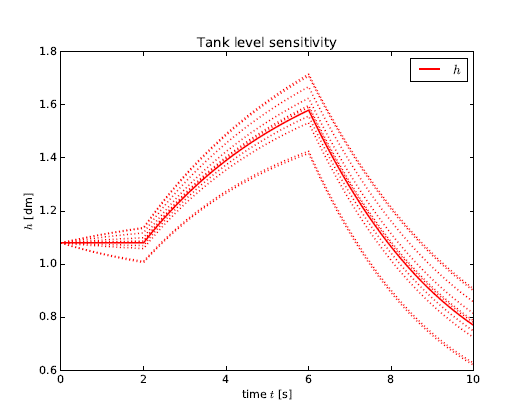
\includegraphics[width=\linewidth]{python_water_tank_level_sensitivity_plot.png}
	\caption{Uncertainty in tank level with a 5\% uncertainty in valve constant $K$. The input is the same as in Figure \ref{fig:pythonwatertanklevelplot}}
	\label{fig:pythonwatertanklevelsensitivityplot}
\end{figure}

\subsection{Parameter Sensitivity/Monte Carlo Simulation}
\label{subsec:pythonparametersensitivity}

It is of interest to study how the model behavior varies with varying uncertain parameter values, e.g., the effluent
valve constant $K$. This can be done as follows:

\begin{lstlisting}
	>>> par = tank.getParameters()
	>>> K = par['K']
	>>> KK = K + (nr.randn(10)-0.5)*K/20
	>>> tank.simulate()
	>>> tm, h = tank.getSolutions('time','h')
	>>> plt.plot(tm,h,linewidth = LW,color = 'red', label=r'$h$')
	>>> for k in KK:
		tank.setParameters(K=k);
		tank.simulate()
		tm, h = tank.getSolutions('time','h')
		plt.plot(tm,h,linewidth=LW,
		color='red',linestyle='dotted',label='_nolabel_')
	>>> plt.title('Tank level sensitivity')
	>>> plt.xlabel(r'time $t$ [s]')
	>>> plt.ylabel(r'$h$ [dm]')
	>>> plt.legend()
\end{lstlisting}

The result is shown in Figure \ref{fig:pythonwatertanklevelsensitivityplot}.

\section{Integration of Wolfram SystemModeler Simulator in PySimulator}
\label{sec:pythonwolframplugin}

PySimulator supports simulation of models in FMU form or using different Modelica tools via extension
plugins. Simulator plugins for tools such as Dymola, SimulationX, and OpenModelica are available from previous work. 
This section presents a new simulator plugin developed for Wolfram SystemModeler.

\begin{figure}
	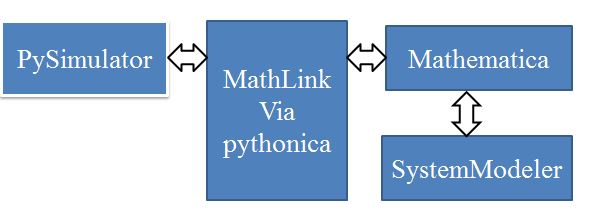
\includegraphics[width=\linewidth]{python_wolfram_communication.png}
	\caption{Communication setup with SystemModeler.}
	\label{fig:pythonwolframcommunication}
\end{figure}

Wolfram SystemModeler has its own symbolic mathematical computation program, Mathematica \cite{mathematica}, which can be used
to perform actions via the Wolfram SystemModeler link (WSMLink) API \cite{wsmlink}, such as loading, compilation and 
simulation of models, or plotting of results. WSMLink provides functionality for integrating Wolfram SystemModeler and Mathematica  
with complete access to models and simulations.

Wolfram SystemModeler can be interfaced to other tools via MathLink \cite{mathlink}, which is a library of functions that 
implement a protocol for sending and receiving Mathematica expressions. MathLink \cite{mathlinktutorial,mathlink} allows external
programs to both call Mathematica and be called by Mathematica. It is possible to create a front end that 
implements your own user interface and communicates with the Mathematica kernel via MathLink \cite{mathlinkc}.

Using the existing interface for simulator plugins in PySimulator, a new simulator plugin has
been implemented: the Wolfram plugin. It enables PySimulator to load and numerically simulate
Modelica models using Wolfram SystemModeler.

The Wolfram plugin is integrated into PySimulator via MathLink and Pythonica \cite{pythonica}, which connects to Mathematica and
SystemModeler. We used the Wolfram SystemModeler API to support loading a Modelica model, simulating
it, and reading the simulation setting file (\textit{.sim}), which is an XML file, to build the variable tree in the
variables browser of PySimulator. The overall communication setup with SystemModeler is given in
Figure \ref{fig:pythonwolframcommunication}.

All of the simulator plugins of PySimulator are controlled by the same Integrator Control GUI. The Wolfram
SystemModeler simulator supports five different numerical integration methods (\textit{DASSL, CVODES,
Euler, RungeKutta, and Heun}), all the simulation menu options are supported (\textit{error tolerance, fixed step
size}, etc.), see Figure \ref{fig:pythonintegratorcontrol}.

\begin{figure}
	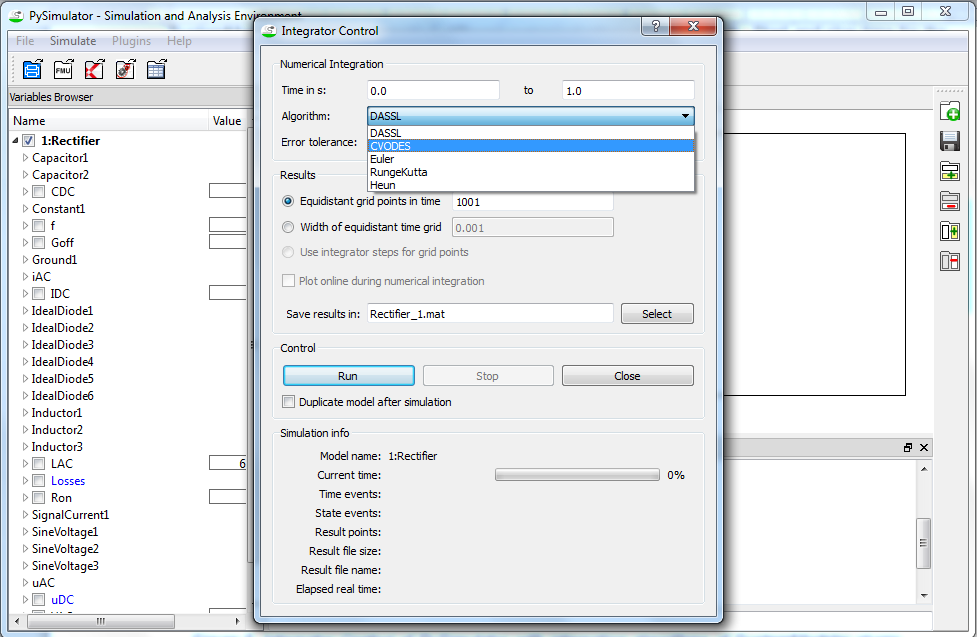
\includegraphics[width=\linewidth]{python_integrator_control.png}
	\caption{Integrator Control of PySimulator with integration algorithms of SystemModeler plugin.}
	\label{fig:pythonintegratorcontrol}
\end{figure}

The \textit{start} and \textit{stop time} for the integration algorithm can be changed and one of the integration algorithms
can be selected. Depending on the integration algorithms the user can change the \textit{error tolerance} or the \textit{fixed step size}
before running the simulation.

It is also possible to simulate the list of models using the Wolfram plugin. The existing PySimulator interface automatically 
includes the new plugin in the simulators list for simulating a list of models.

\begin{landscape}
\begin{figure}
	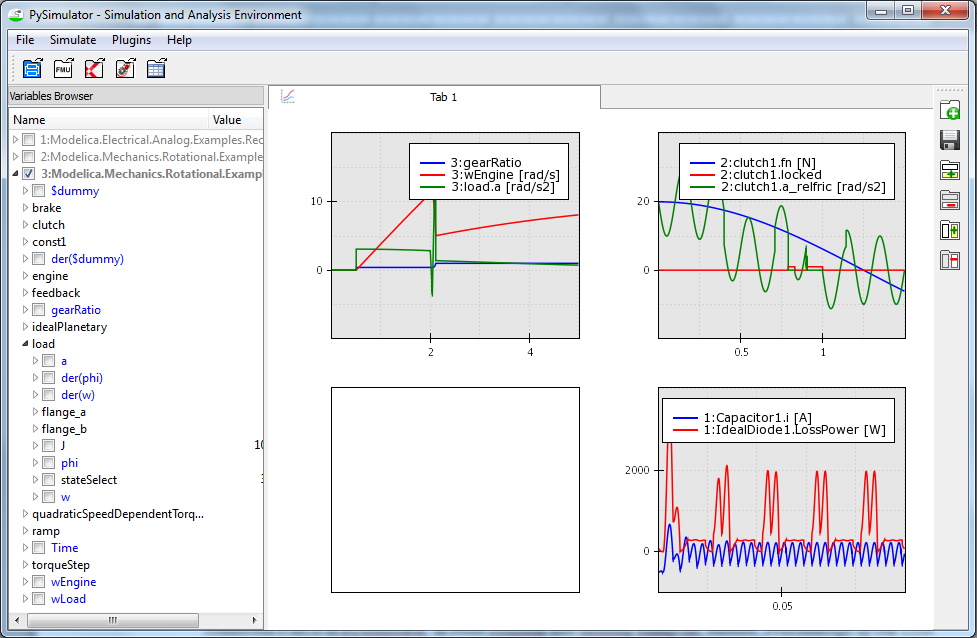
\includegraphics[width=\linewidth]{python_list_of_simulate_models.png}
	\caption{List of simulate models via Wolfram plugin.}
	\label{fig:pythonlistofsimulatemodels}
\end{figure}
\end{landscape}

\section{Summary}
\label{sec:pythonsummary}

In this chapter, we have introduced an enhanced Python interface for interacting with FMUs and Modelica models for further analysis and post-processing of simulation results. We have presented how a modeler can use the Python interface to simulate and access Modelica models using Python objects. The idea behind this interface is to provide the modeler with the ability to manipulate and exchange data with Modelica models before and after simulations. A case study of a Modelica model is presented to illustrate the tool’s usage.

We have also presented a simulator plugin for a commercial simulation engine for Modelica models - the Wolfram SystemModeler within PySimulator. The existing PySimulator interface automatically includes the new plugin in the simulators list for simulating lists of models. We have successfully tested by loading all of the result files generated from the Wolfram plugin and verified the results by comparing with several other base line tools. The integration of the Wolfram SystemModeler simulator plugin uses the regression analysis framework within PySimulator to compare results of the same model generated from SystemModeler with several other tools or different versions of the same model from the SystemModeler tool.

\subsection*{Acknowledgments}
\label{sec:pythonacknowledgments}

Part of the PySimulator work is financed by the CleanSky Joint Undertaking project PyModSimA (JTI-CS-2013-2-
SGO-02-064). This support is highly appreciated. The authors thank Jakub Tobolar (DLR
Institute of System Dynamics and Control) for his tests and support of the regression testing feature in an
earlier stage and his implementation of the automatic generation of the simulation setup file by Dymola.

%\nocite{scigen}
%We have included Paper \ref{art:scigen}

%%%%%%%%%%%%%%%%%%%%%%%%%%%%%%%%%%%%%%%%%%%%%%%%%%%%%%%%%%%%%%%%%%%%%%
%%% Intro.tex ends here


%%% Local Variables: 
%%% mode: latex
%%% TeX-master: "demothesis"
%%% End: 

